\section{Deep models detail}
\label{sec:Deep models detail}
% 8 pages
Machine learning is a branch of artificial intelligence. Deep learning is also a branch of machine learning, which utilises artificial neural networks for feature learning and hierarchical feature extraction to replace manual feature engineering in other machine learning methods.
Recently, the research of deep learning is a hot topic in the field of computer science, and it is also an important method used in the computer vision task in this research.
This section will introduce the details of a variety of deep learning models related to this research, including CNN, RNN, attention and Transformer structures.
Although the applications or target tasks of these models are different, the design ideas between them are mutually influential.
Therefore, reviewing the development and design concepts of these previous models will greatly help the design of the model in this research.

\subsection{Convolutional neural network} % 2.5 pages
With the rapid development of neurobiology and cognitive science, the concept of artificial neural networks, a computational model that imitates the structure and function of biological neural networks, has been proposed as early as the last century.
\citet{fukushima1980neocognitron} proposes a network created from the animal visual system as well as some key concepts, such as \textbf{local receptive field}, \textbf{multi-layer perception architecture} and translation \textbf{equivariance and invariance property} (not affected by shift in position).

In detail, the local receptive field means that each neuron will not perceive the image as a whole, but will only perceive the local information, then the local perception can be integrated through a multi-layer perception architecture to obtain the global perception.
On the other hand, the property of translation equivariance and invariance is emerging from the combination of the local receptive field and multi-layer perception architecture.

The study of neurobiology and cognitive science is then evolved into a computational model. For example, \citet{zhang1988shift} propose the first two-dimensional Shift Invariant Artificial Neural Network (SIANN).
Then, \citet{lecun1989backpropagation} propose a original CNN with two convolutional layers and two fully connected layers using backpropagation method to train in a supervised learning approach.
They also highlight the term convolution for the first time, and named this model type as convolutional neural network (CNN).
Soon after the application of this model in handwritten zip code recognition, \citet{zhang1994computerized} apply it to a practical case of recognising medical imagery.

\begin{figure}[ht!]
    \centering
    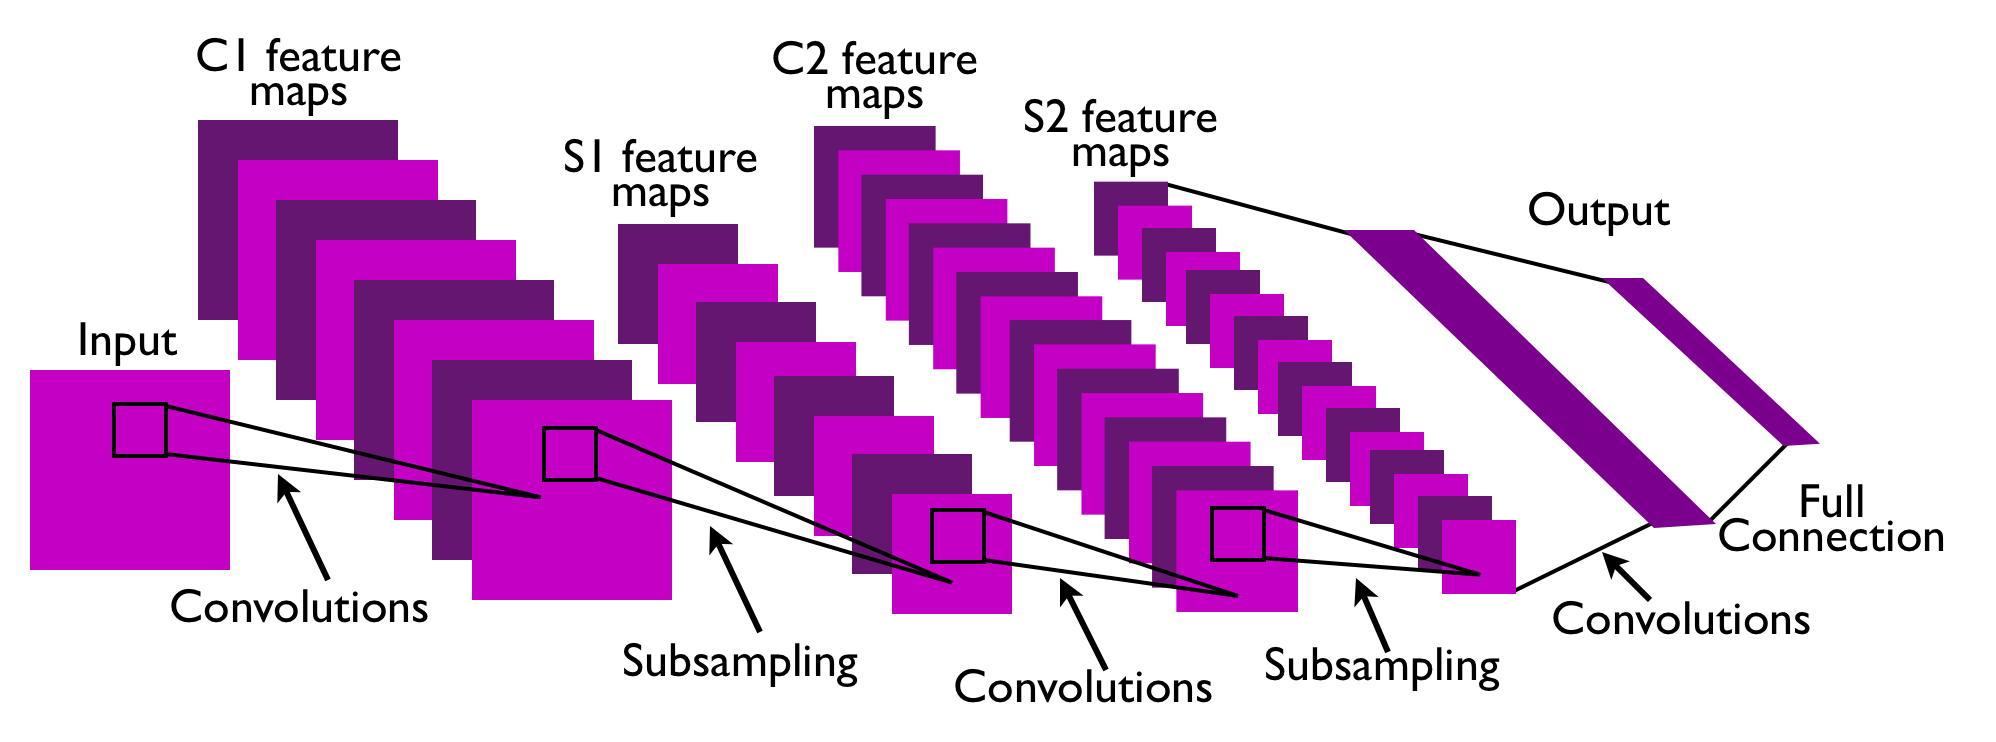
\includegraphics[width=\textwidth]{literature/imgs/ext-lecun-cnn-arch.png}
    \caption{CNN applications in vision by \citet{lecun2010convolutional}}
    \label{fig:ext-lecun-cnn-arch}
\end{figure}

The most revolutionary progress is that \citet{lecun2010convolutional} propose a modern architecture for this model, as illustrated in figure \ref{fig:ext-lecun-cnn-arch}.
This structure comprises three convolutional layers combined in between with two sub-sampling layers, and two fully connected layers. Sub-sampling, also known as pooling, reduces the size of feature maps, by retaining only important information to simplify calculation.
Further, it further strengthens the translation invariance, taking maximum pooling as example, because the translation does not affect the maximum value, the pooling result remains unchanged.

In the following years of development of CNN, the number of layers in deep networks is gradually deepening to obtain greater high-level information.
In 2012, \citet{krizhevsky2012imagenet} propose AlexNet which use 5 convolutional layers and 3 fully connected layers.
However, as the number of hidden layers increases, the model gets more complex and prone to overfitting.
AlexNet uses the Dropout layer by randomly breaking neuron connection (setting random input units to zero) in training process to prevent overfitting. 
Two years later, \citet{simonyan2014very} propose Visual Geometry Group (VGG) model, in which $3\times3$ size convolution kernels are fully used in a total of 5 layers, just as the title of the paper, it is a very deep convolutional network.

The experiment in the VGG model concludes that the deeper the number of network layers, the better the performance.
However, as the depth of the model and the number of parameters continue to increase, the following two significant problems have been discovered.

\begin{enumerate}
    \item The network is prone to overfit, requiring more training data, making it more difficult to train.
    \item More storage resources and computing resources are required, but cannot provide adequate performance boost. 
\end{enumerate}

In order to solve these problems, \citet{he2015deep} propose a residual structure to make deep network training easier with enhanced performance but fewer parameters and lower complexity. 
They first identify that the root cause of these problems is that the deeper network structure leads to degradation, i.e., the training error and the verification error both increase since the deeper network does not learn anything but loses useful features.
Then, figure \ref{fig:ext-CNN-ResNet-BBs} illustrates two types of building blocks used in ResNets with different number of layers.
The first typical block just uses cross-layer connection, a linear layer from input to output connected directly.
By denoting the desired underlying mapping as $H(x)$, the each layer learns the residual between input $x$ and desired output $F(x):=H(x)-x$.
As a result, such a residual structure allows the deep network to adapt to the appropriate depth, i.e., use the identity transform across unnecessary layers.

Further, figure \ref{fig:ext-CNN-ResNet} compares the network structure of VGG-19, 34-layer plain, and 34-layer residual and shows how to use the building block in the actual deep network. 
Figure \ref{fig:ext-CNN-ResNet-BBs} also shows a ``bottleneck'' building block for deeper ResNets, which first uses a $1\times1$ size convolution to reduce the dimensional across channels to reduce the calculation required in the $3\times3$ convolution.

\begin{minipage}[ht]{.32\textwidth}
    \begin{figure}[H]
        \centering
    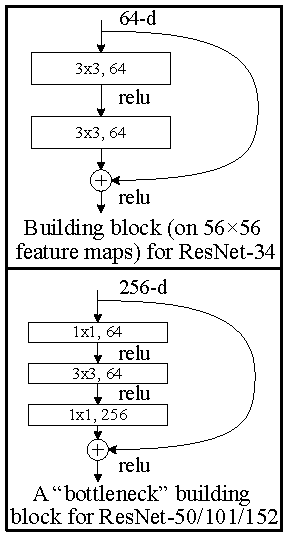
\includegraphics[width=.99\textwidth]{literature/imgs/ext-CNN-ResNet-BBs.pdf}
    \caption{Residual building blocks by \citet{he2015deep}}
    \label{fig:ext-CNN-ResNet-BBs}
    \end{figure}
\end{minipage}
\hspace{1em}
\begin{minipage}[ht]{.62\textwidth}
    \begin{figure}[H]
        \centering
    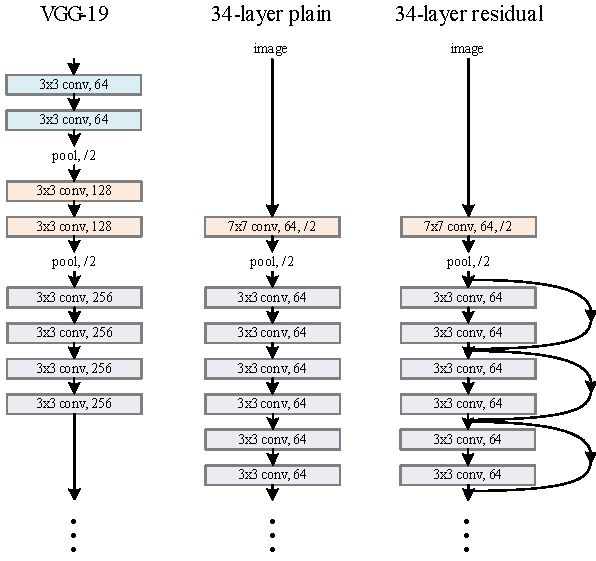
\includegraphics[width=.99\textwidth]{literature/imgs/ext-CNN-ResNet.pdf}
    \caption{VGG and Residual ImageNet by \citet{he2015deep}}
    \label{fig:ext-CNN-ResNet}
    \end{figure}
\end{minipage} %2.5

\subsection{Recurrent neural network} % 2.5 pages
CNN solves the spatial problem of imagery and has been widely used in the field of computer vision, but it is powerless for data with time-series features.
For example, it is necessary to understand the words sequentially in sentences in natural language processing tasks.
And in understanding videos, it is necessary to understand the relationship between frames.
In these tasks, the recurrent neural network (RNN) emerged to process the time-series features.

\citet{jordan1986serial} proposed the Jordan network, by introducing a recurrent connection that feeds back the output of the whole network to the input layer after a time delay.
Later in 1990, \citet{elman1990finding} formally defined the recurrent neural network model, in which the output of each recurrent hidden layer goes to the subsequent layers and feeds back to the input of the layer after a time delay.
The first figure on the left in Figure \ref{fig:2-RNN-unfold} shows the structure of the simplest recurrent network, with an input-output and a hidden layer, denoted as $x$, $y$ and $h$, where the arrows indicate the flow of data.

The middle unfolded RNN figure shows the sequential structures by unfolding inputs and outputs of the network in chronological order. 
The input includes the initial hidden state $a^0$, a series of data $x^n$, then the model generates sequential outputs $y^n$. However, the model with unidirectional memory has a limitation that the model can only know the history data and cannot foresee the data that is about to be input.
For tasks requiring two-way dependencies, such as natural language processing, each word has a strong relationship associated with other surrounding words, thus a bidirectional RNN structure is introduced as shown in the right figure in Figure \ref{fig:2-RNN-unfold}.

\begin{figure}[ht!]
    \centering
    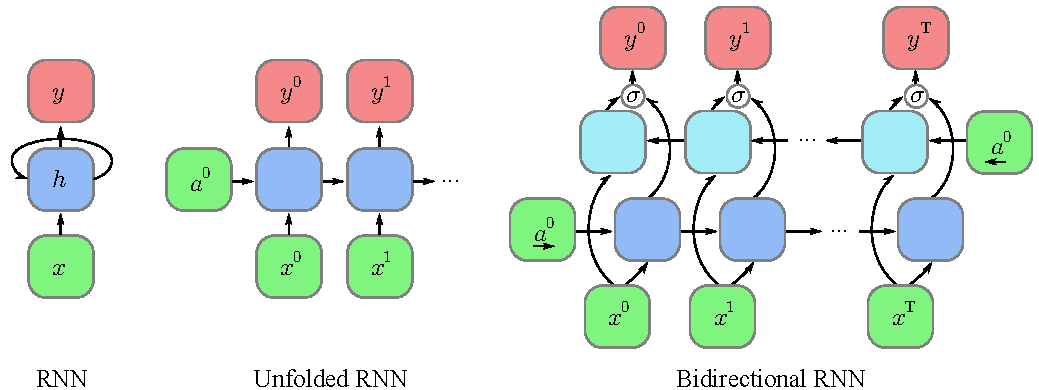
\includegraphics[width=\textwidth]{literature/imgs/2-RNN-unfold.pdf}
    \caption{RNN, unfolded unidirectional RNN and unfolded bidirectional RNN}
    \label{fig:2-RNN-unfold}
\end{figure}

%LSTM
However, \citet{hochreiter1997long} pointed out that simple RNN tends to only keep short-term memory and is prone to lose long-term memory, because the same weight of the network is shared at all time steps, and the final gradient tends to disappear after multiple time steps, proved by Hochreiter's analysis.

\begin{equation}
    \frac{\partial \vartheta_{v}(t-q)}{\partial \vartheta_{u}(t)}=\sum_{l_{1}=1}^{n} \ldots \sum_{l_{q-1}=1}^{n} \prod_{m=1}^{q} f_{l_{m}}^{\prime}\left(n e t_{l_{m}}(t-m)\right) w_{l_{m} l_{m-1}}
    \eqcite{hochreiter1997long}
    \label{equ:2-RNN-loss-scaled}
\end{equation}

Formula \ref{equ:2-RNN-loss-scaled} shows that the back-propagation gradient in simple RNN is equal to the product of the gradients of each time step after multi-step propagation.
An intuitive explanation is that the gradient is mainly dominated by the short-distance gradient, and thus it is difficult for the model to learn long-distance dependence.

Long-short-term memory (LSTM) was proposed to solve the problem that the simple RNN cannot learn long-term dependence by introducing a separated cell state $C_t$ to keep long-term memory. And later on, \citet{Gers2000LearningTF} introduced I/O gates, a forget gate to control loss or keep memory in cell state, resulted in the modern LSTM cell structure shown in the left of Figure \ref{fig:ext-LSTM-GRU}.

\begin{figure}[ht!]
    \centering
    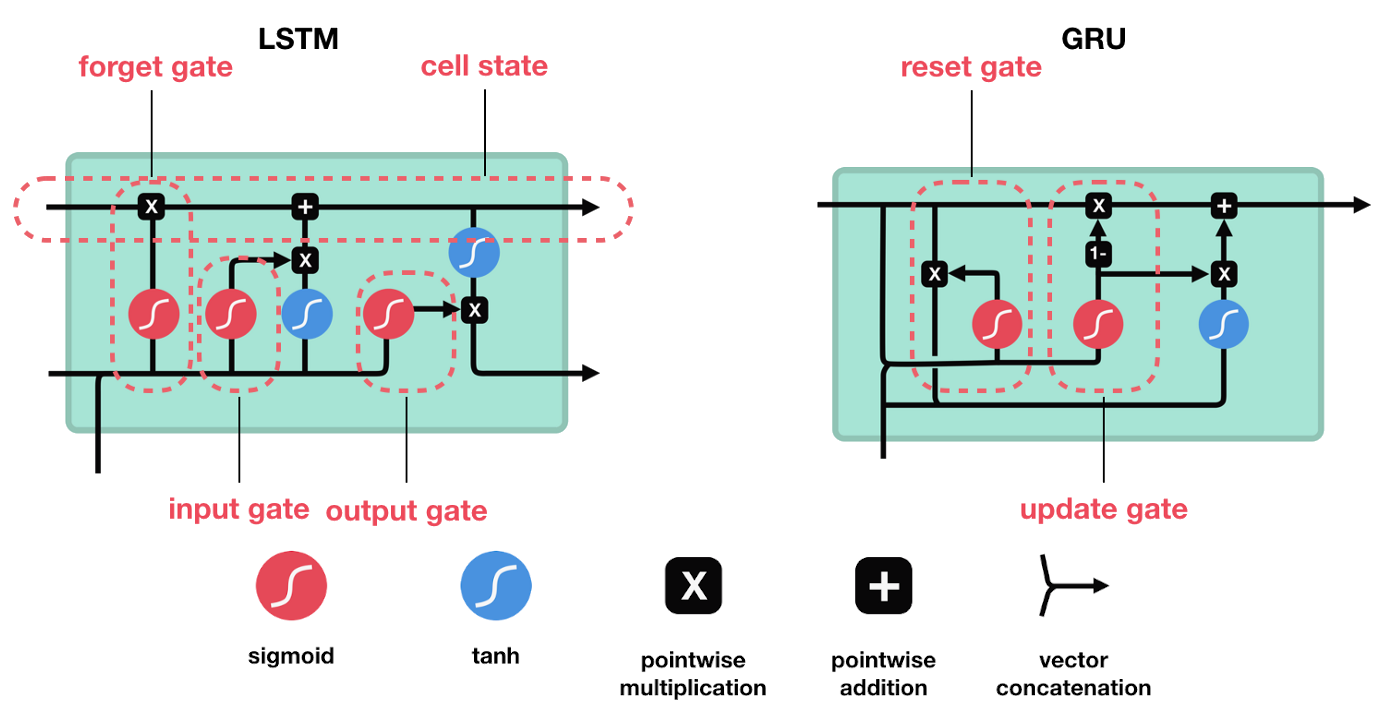
\includegraphics[width=.9\textwidth]{literature/imgs/ext-LSTM-GRU.png}
    \caption{LSTM and GRU structure comparison by \citet{phi2018illustrated}}
    \label{fig:ext-LSTM-GRU}
\end{figure}

%GRU
LSTM introduces lots of things into RNN, which leads to an increase in trainable parameters of each unit, making it harder to create a model with a deeper network.
Gated recurrent unit (GRU) is an improved LSTM algorithm proposed by \citet{chung2014empirical} in 2014. It merges the forget gate and the input gate into a single update gate. It also combines the cell state and the hidden state.
As shown in the right of Figure \ref{fig:ext-LSTM-GRU}, GRU structure is much simpler than LSTM, making it possible to create a deeper network.

LSTM and GRU only remedy and alleviate the problem of gradient vanish to a certain extent in RNN, and memory loss can still occur in the case of long-range dependencies.
Most importantly, this network structure has one limitation that made it not suitable for mobile applications.
The enforced sequential calculation process is due to dependencies on the result from the previous time, which greatly limits the parallel capability of calculations, thus making it impossible to achieve reasonable performance on mobile devices.
 %2

\subsection{Attention and Transformer} % 2.5 pages
The attention mechanism originated from the human experience of perceiving things either visually or audibly.
Intuitively speaking, when we observe something through sight, we do not pay attention to all the details but paying attention to a certain part that needs to be focused and giving low attention to the surroundings.

The attention mechanism was firstly added to recurrent neural networks as a visual attention modelling.
In 2014, \citet{mnih2014recurrent} proposed a recurrent attention model that combined ideas in RNN and the attention mechanism for image classification and achieved good performance.
Besides, the researchers discussed and reached forward-looking conclusions that it can be used in object recognition and video classification in future work due to the encouraging results achieved.

In 2016, \citet{bahdanau2016neural} firstly introduced the attention mechanism into the natural language processing field.
In their work, they perform translation and alignment jointly with the attention mechanism on machine translation tasks because ``the use of a fixed-length vector is a bottleneck in improving the performance of this basic encoder-decoder architecture'', said by \citet{bahdanau2016neural}.

\begin{minipage}[]{\textwidth}
\centering
\begin{minipage}[ht]{.35\textwidth}
    \centering
    \begin{figure}[H]
        \centering
        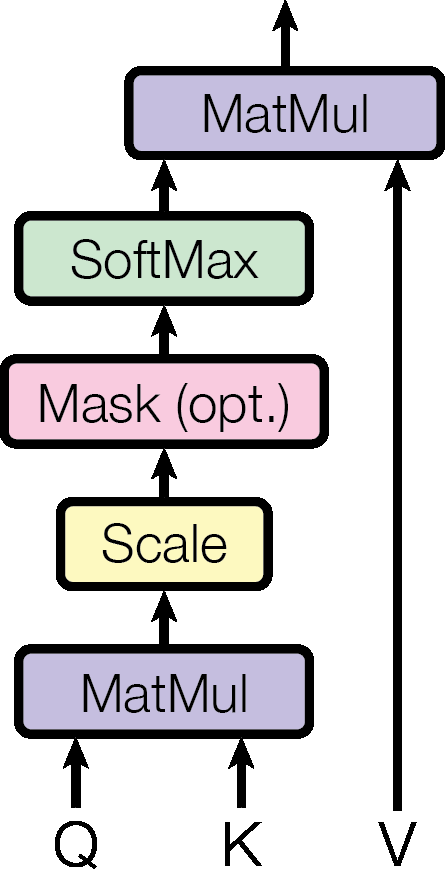
\includegraphics[width=.48\textwidth]{literature/imgs/ext-attention-dot-product.png}
        \caption{Scaled Dot-Product Attention \cite{vaswani2017attention}}
        \label{fig:ext-attention-dot-product}
    \end{figure}
    \vspace*{-.5cm}
    \begin{figure}[H]
        \centering
        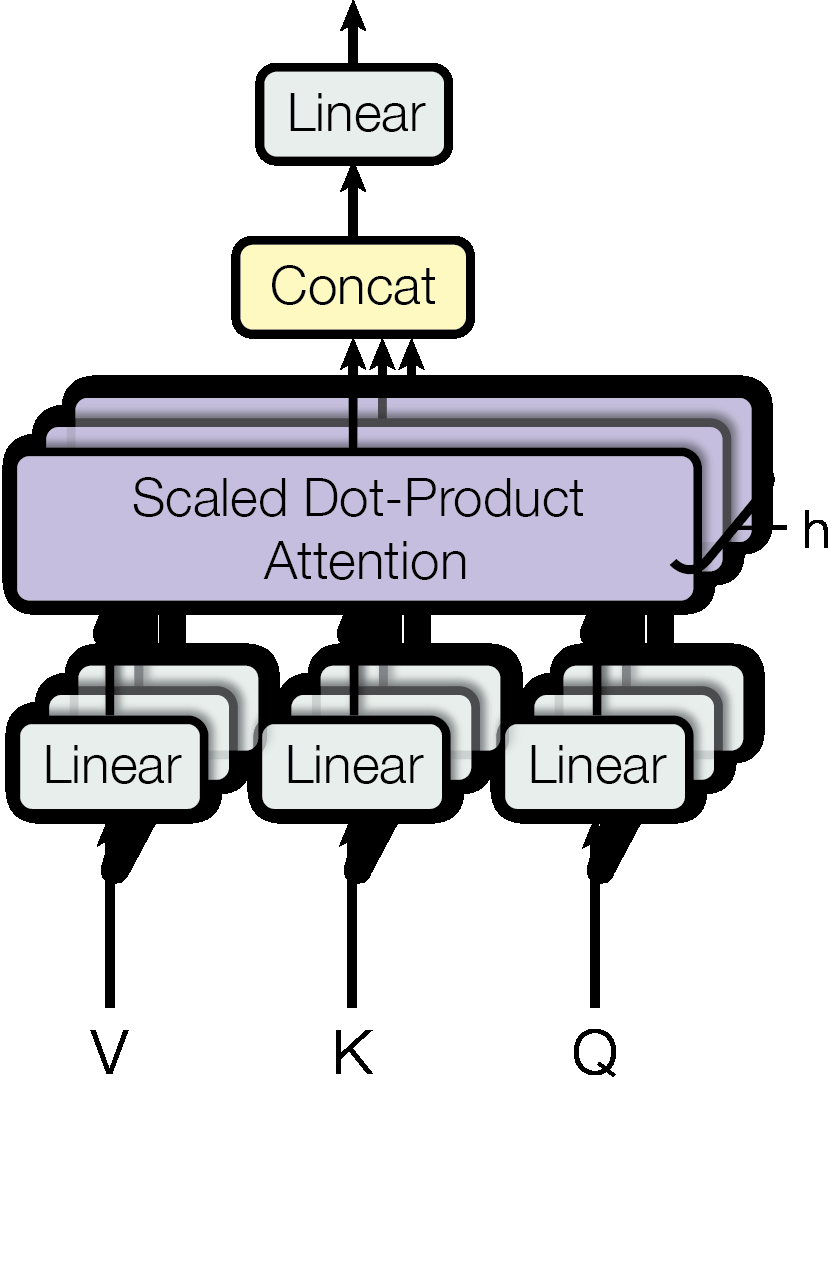
\includegraphics[width=.9\textwidth]{literature/imgs/ext-attention-multihead.png}
        \vspace*{-2em}
        \caption{Multi-Head Attention \cite{vaswani2017attention}}
        \label{fig:ext-attention-multihead}
    \end{figure}
\end{minipage}
\hspace{1em}
\begin{minipage}[ht]{.52\textwidth}
    \begin{figure}[H]
        \centering
        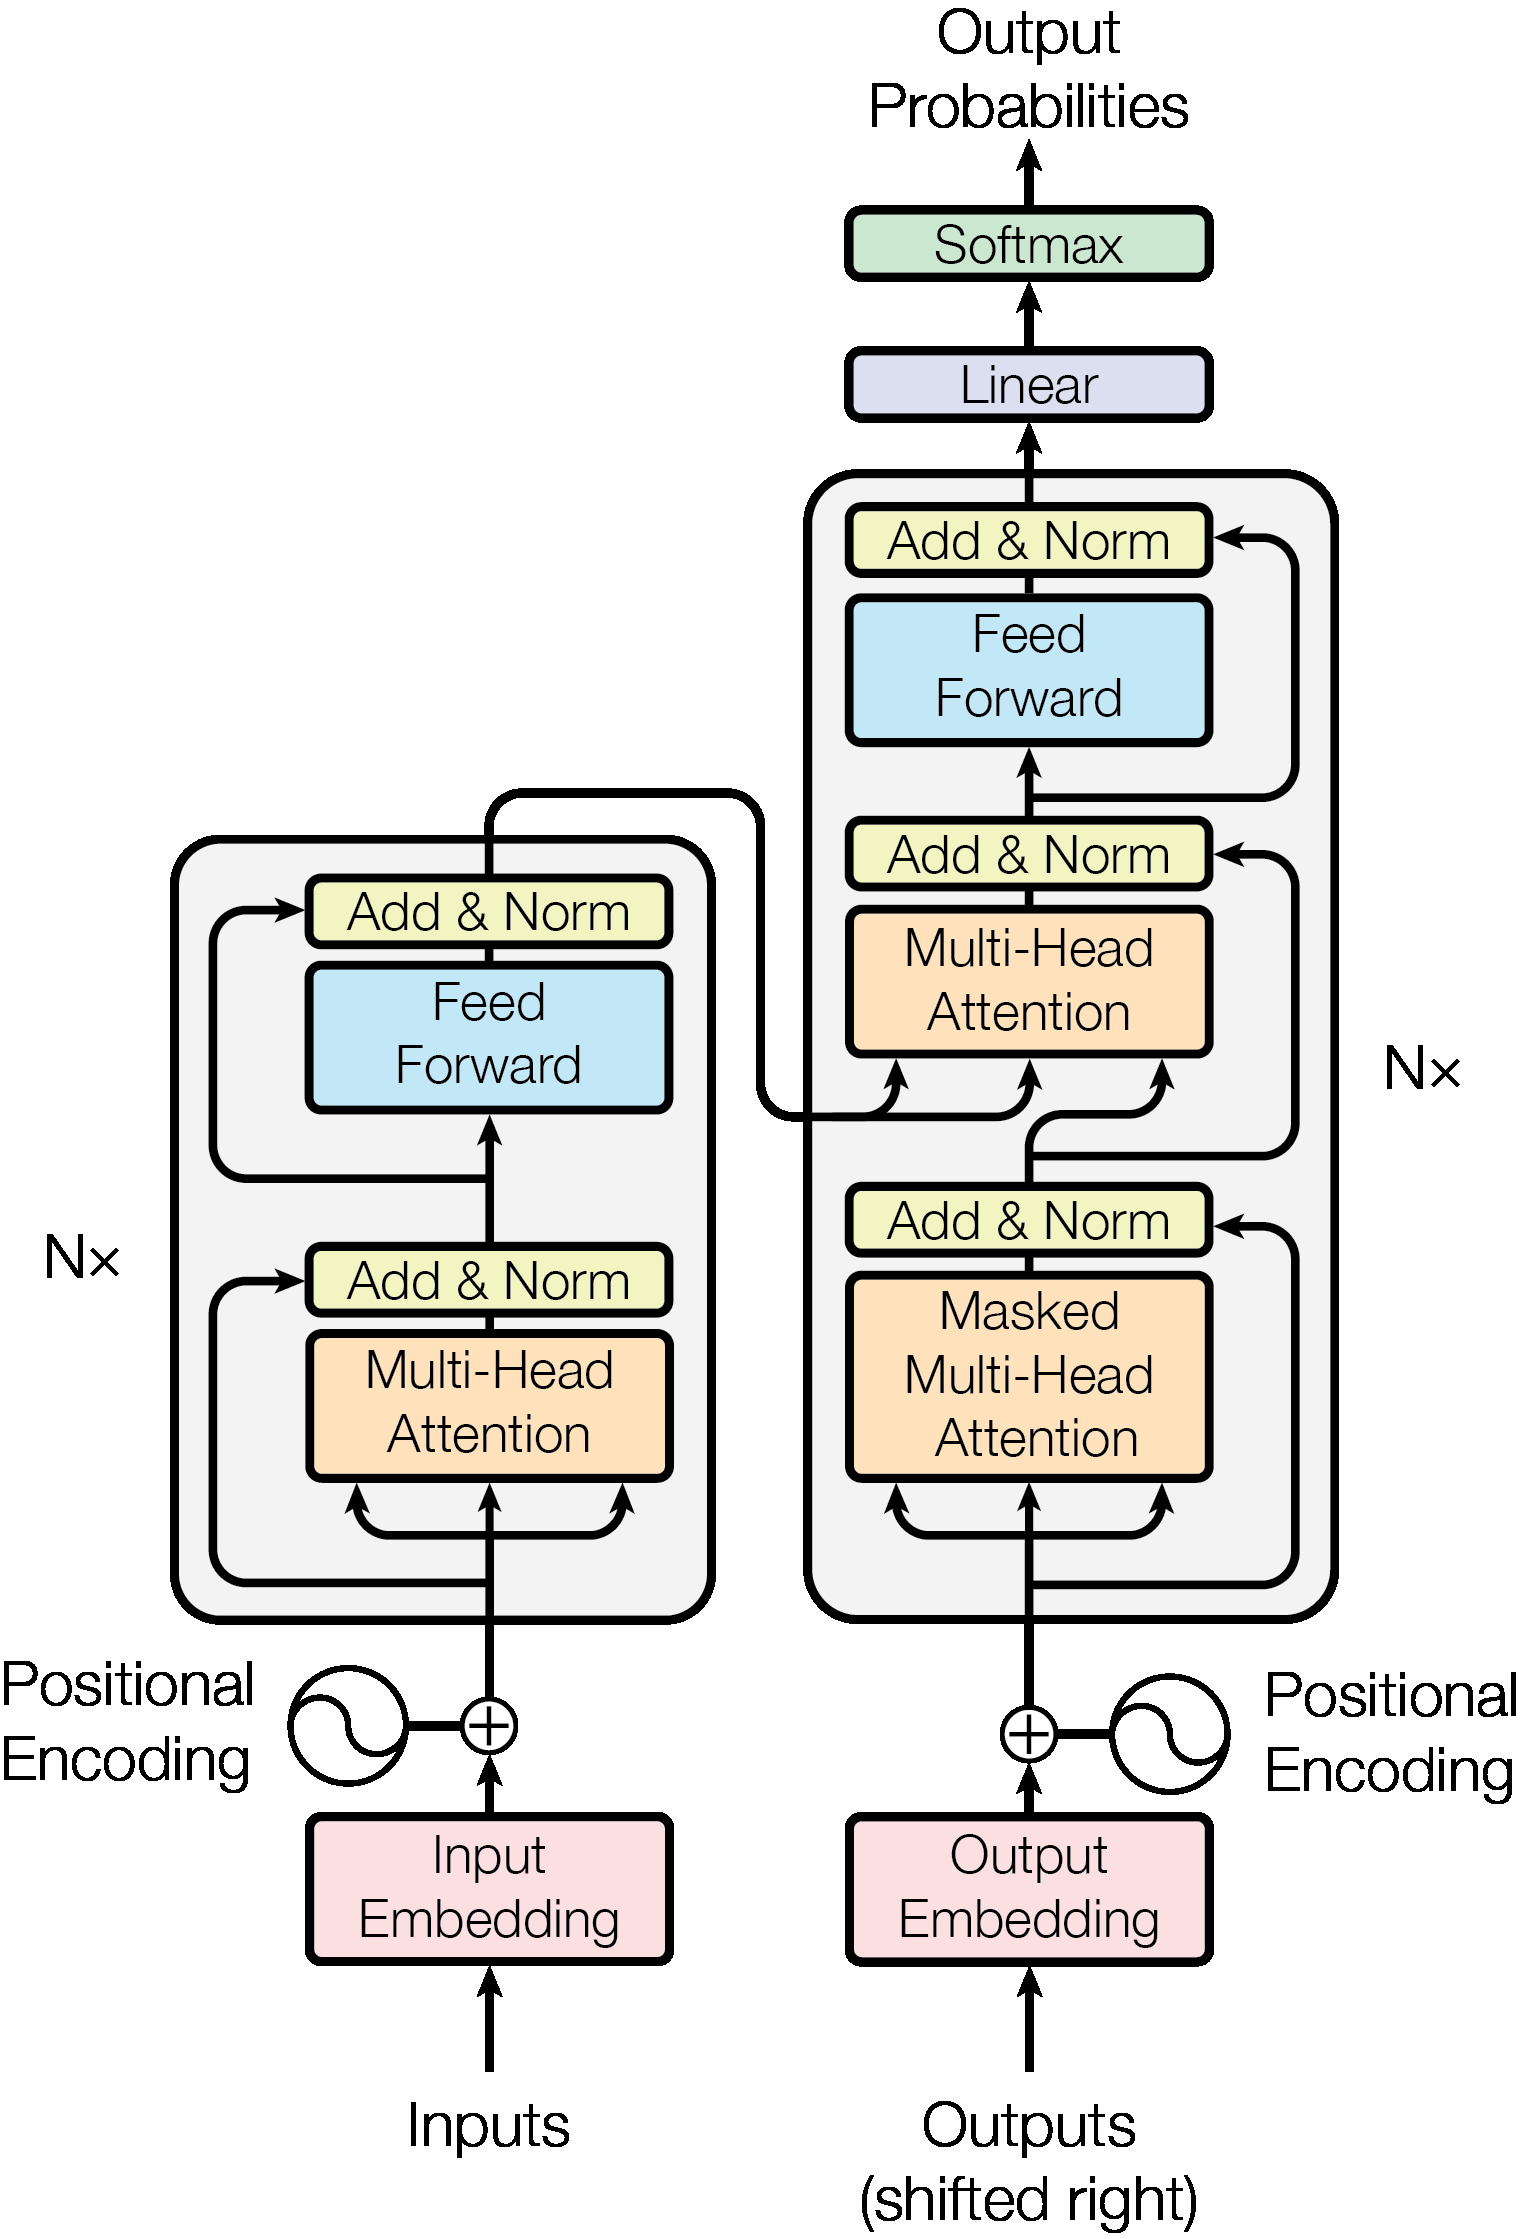
\includegraphics[width=\textwidth]{literature/imgs/ext-transformer.png}
        \caption{The Transformer model architecture \cite{vaswani2017attention}}
        \label{fig:ext-transformer}
    \end{figure}
\end{minipage}
\end{minipage}

One year after the attention mechanism was applied in the machine translation tasks, \citet{vaswani2017attention} proposed scaled dot-product attention (Figure \ref{fig:ext-attention-dot-product}), multi-head attention (Figure \ref{fig:ext-attention-multihead}) and the Transformer model (Figure \ref{fig:ext-transformer}) that is ``relying entirely on self-attention to compute representations of its input and output without using sequence aligned RNNs or convolution'', said by \citet{vaswani2017attention}.
Then, experiments were performed on the machine translation task using the proposed Transformer model and achieved better performance and results, making the attention mechanism the most preferred solution for natural language processing tasks.

\begin{equation}
    Attention(Q, K, V) = softmax(\frac{QK^T}{\sqrt{d_k}})V
    \eqcite{vaswani2017attention}
    \label{equ:2-attention}
\end{equation}

Figure \ref{fig:ext-attention-dot-product} shows the scaled dot-product attention mechanism, where Q, K, and V represent Query, Key and Value respectively.
Further, formula \ref{equ:2-attention} shows the calculation process of it mathematically.
In this formula, the dot-product between Query and Key matrix represents their similarity, which is normalised by the square root of the dimension of $d_k$, since dot-product may grow large in magnitude, pushing the softmax activation function into regions where it has extremely small gradients.
The result from softmax activation is normalised probabilities representing the attention matrix visualised in Figure  \ref{fig:ext-attention_map_portuguese}.

\begin{figure}[!ht]
    \centering
    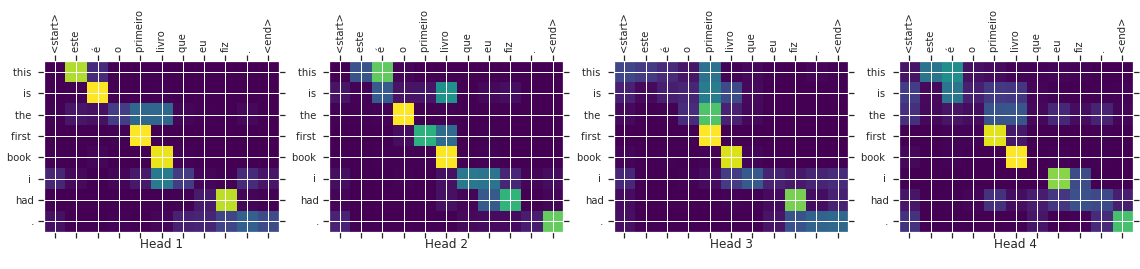
\includegraphics[width=\textwidth]{literature/imgs/ext-attention_map_portuguese.png}
    \caption{Multi-head attention matrix visualisation \cite{tensorflow2021transformer}}
    \label{fig:ext-attention_map_portuguese}
\end{figure}

The idea behinds multi-head attention is like using multiple kernels in CNN to capture different features.

%Transformer
While convolutional neural network (CNN) is in the ascendant among the fields of computer vision, transformer model composed of self-attention structures has achieved state-of-the-art results in many natural language processing tasks.

\citet{devlin2019bert}

The transformer model gradually replaced the recurrent neural network (RRN) with sequential computing restriction and long-term memory loss issues.

Innovative design concepts from the transformer model are also carried forward in the fields of computer vision.

Many recent studies, such as Data-efficient image Transformers (DeiT) and Shifted window (Swin) transformers, have improved widely-adopted CNN-only models such as VGG and ResNet by introducing the self-attention structures to achieve better performance.

\citet{dai2021coatnet}

\citet{guo2021cmt} %3.5
